\chapter{设计原理}\label{sec:theory}

本节介绍本设计的理论框架,包括 Spring 框架、数据库设计与优化技术以及视频压制优化技术等。

\section{Spring 框架}

近年来 Spring 框架是 Java Web 框架中经常被使用的,其主要目的是降低应用系统开发时的复杂性。Spring 框架构建基于其核心,Spring 核心模块提供了一个 IoC 容器以及一些举出工具类。Spring AOP 模块位于核心模块之上,这为开发者提供了一系列面向切面编程支持。在 AOP 模块之上是数据访问与事务管理功能\cite{walls2005spring}。下文将详细介绍这三个 Spring 框架的基础功能。

\subsection{Spring 框架的控制反转容器}

控制反转 (Inversion of Control, IoC) 概念来源于依赖倒置原则。依赖倒置原则即高层模块不应该依赖低层模块,二者都应该依赖其抽象;抽象不应该依赖细节;细节应该依赖抽象\cite{gamma1995design}。简单地说,高层模块与低层模块不应该直接产生耦合,高层与低层模块应通过一个接口耦合在一起,即高层模块依赖于该接口,低层模块实现该接口。如图 \ref{fig:beforeAndAfter} 所示,这样对于低层模块的修改就不会对高层模块产生较大的影响同时也减小了系统各模块的耦合。

\begin{figure}[!ht]
\centering
\subfloat[使用 IoC 前]{
	\centering
	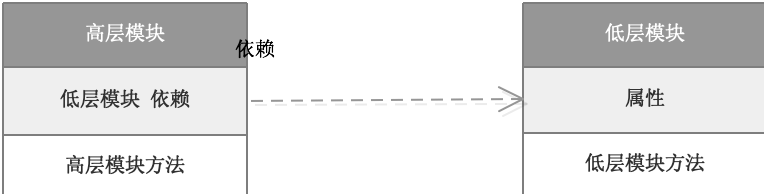
\includegraphics[width=0.5\textwidth]{beIOC.png}}\quad
\subfloat[使用 IoC 后]{\centering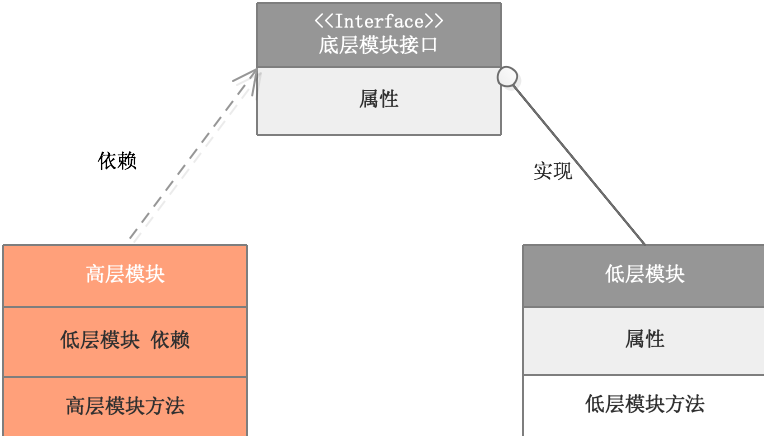
\includegraphics[width=0.5\textwidth]{afIOC.png}}
\caption{使用 IoC 前后 UML 图}
\label{fig:beforeAndAfter}
\end{figure}

Spring 的控制反转容器是通过依赖注入 (Dependency Injection, DI) 实现的。如图 \ref{fig:DI} 所示,依赖注入即高层模块在使用低层依赖时,不是自己将低层模块实例化而是向控制反转容器申请一个已创建好的依赖对象\cite{prasanna2009dependency}。这样高层模块与低层模块间的耦合被降低了,对于低层模块的改变对高层模块产生的影响也变小了。同时,由于低层模块由容器创建,我们就可以轻松地实现单例模式等设计模式,进一步简化了开发也提高了系统的性能。

\begin{figure}[!ht]
    \centering
    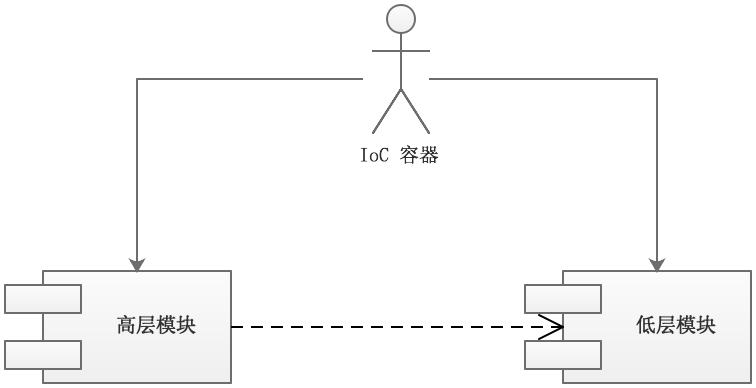
\includegraphics[width=0.6\textwidth]{IoC.png}
    \caption{Spring 依赖注入作用}
    \label{fig:DI}
\end{figure}

通过使用 Spring 框架提供的 IoC 容器,我们可以轻松地使用控制反转构建应用系统。

\subsection{Spring AOP 框架}

在一个应用系统中存在着一些许多模块公用的功能,如:日志记录、安全检查以及事务功能等。这些公用功能如果处置不当就会造成系统的代码冗余度增加和耦合性上升,例如:要在系统中增加一次日志记录,我们就必须在所有的模块中加入相同的代码,着无疑是非常低效的。对此,我们可以使用面向切面编程 (Aspect Oriented Programming) 来解决这一问题。

\begin{figure}[!ht]
    \centering
    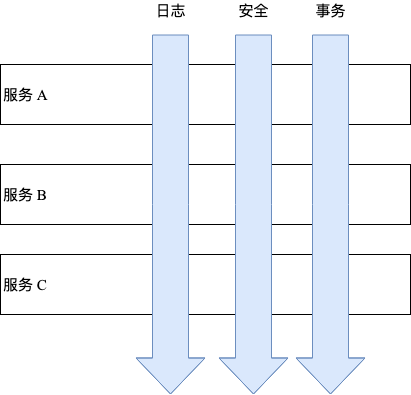
\includegraphics[width=0.4\textwidth]{AOP.png}
    \caption{面向切面编程中的横切关注点}
    \label{fig:AOP}
\end{figure}

如图 \ref{fig:AOP} 所示,面向切面编程可以将系统中的公共功能抽象成为许多称之为横切关注点的功能模块,例如:日志记录功能就是一个横切关注点。系统中需要使用这些公共功能的地方称之为连接点 (Joinpoint)\cite{walls2005spring}。在系统运行时面向切面编程框架会将横切关注点织入连接点中,这样系统就可以使用所有的公共功能,减少了系统的冗余代码与耦合性。

Spring 框架中的面向切面编程功能由动态代理实现,源于设计模式中的代理模式。如图 \ref{fig:Proxy} 所示,代理模式的作用是为隔离被代理对象,使用代理提供功能调用\cite{gamma1995design}。代理处于访问者与被访问者之间,隔离两者的直接交互。在代理将访问者的访问请求传递给被访问者时,代理可以添加一部分额外的功能,如安全检测。因此,代理模式可以有效地增强系统的灵活性与安全性。动态代理的实现还要依靠 Java 提供的反射功能。反射功能允许我们在 Java 程序的运行期间动态载入类、创建对象以及生成代理。通过实现代理模式、使用反射机制,我们就可以创建出动态代理系统,实现面向接口编程\cite{walls2005spring,walls2016spring}。

\begin{figure}[!ht]
    \centering
    \includegraphics[width=0.6\textwidth]{Proxy.png}
    \caption{代理模式 UML 图}
    \label{fig:Proxy}
\end{figure}

Spring AOP 的设计遵循了 8/2 原则,即通过 20\% 的代码实现 AOP
 框架 80\% 的功能。因此Spring AOP 支持的 AOP 功能是不完全的,例如 Spring AOP 不支持属性级别的拦截等。系统运行时,我们在系统中定义所有的切面、连接点都会被 Spring AOP 拼装起来,这个操作被称为织入\cite{spring2019}。织入时,Spring 会自动生成切面的代理包装类,通过代理包装类将切面织入代码中。Spring AOP 框架为我们提供了 AOP 的大部分功能,同时我们也可以整合使用 AspectJ 等框架来获取 Spring AOP 不支持的功能。
 
 \subsection{Spring 事务管理功能}
 
 事务管理的作用是保证应用系统在操作数据库时不会对数据的正确性产生破坏,具体的事务定义将在下文介绍。在 Spring 框架中,我们通常使用声明式的方式使用事务,事务也是一个常用的 AOP 中的横切关注点。通常情况下使用事务,我们需在每次访问数据库前声明事务开始,在事务正常结束后进行结束事务操作,在事务异常结束后进行事务的回滚。Spring 框架使用 AOP 来处理事务,通过在运行时将事务代码织入应用中来简化开发\cite{spring2019,walls2005spring}。
 
 我们在需要使用事务的地方使用 @Transactional\cite{spring2019} 注解即可开启声明式事务功能。我们可以在其中设置一些事物属性。事务属性主要包括:隔离级别、传播行为、回滚规则、是否只读以及超时时间等。通过注解使用声明式事务对于简化数据访问层的开发具有较大的意义\cite{walls2016spring}。


\section{数据库的原理与设计}

本次设计采用 MySQL 作为系统主数据库、Redis 作为缓存数据库。


\subsection{关系型数据库}
支持关系模型的数据库系统为关系型数据库系统。关系模型主要数据结构为关系{codd1970relational}。关系中的域是一组具有相同数据类型的值的集合。一个关系可以由多个域的笛卡尔积表示。如一个班中所有学生的年龄的集合就是一个域\cite{王珊2006数据库系统概论}。

笛卡尔积是一种域上的集合运算,其定义为:

\begin{equation}
\label{eq:Descartes}
D_1 \times D_2 \times \cdots \times D_n = {(d_1, d_2, \cdots, d_n) | d_i \in D_i, i=1, 2, \cdots, n}
\end{equation}

其中,每一个元素 $(d_1, d_2, \cdots, d_n)$ 为一个元组。笛卡尔积可以表示一个二维表,表中的一行对应笛卡尔积中的一个元组。$D_1 \times D_2 \times \cdots \times D_n$ 的子集为在域 $D_1, D_2, \cdots, D_n$ 上的关系\cite{codd1970relational}。

每一个关系中都存在一些特殊的属性。若关系中某一属性组可以唯一标志该元组,而其任意子集均无此性质,则该属性组为这个关系的候选码。任意包含在至少一个候选码中的属性为主属性,不包含在所有候选码中的属性为非主属性。在任意关系表中不可能存在具有相同候选码的两个或多个元组\cite{codd1970relational,王珊2006数据库系统概论}。

关系模式可以表示为 $R(U, D, DOM, F)$,其中 $R$ 为关系名,$U$ 为属性名的集合,$D$ 为域的集合,$DOM$ 为属性与域的映射,$F$ 为属性间的依赖关系。关系模式中主要包含关系中有哪些属性、关系中有哪些域以及域与属性的映射关系。

关系数据模型中具有关系的操作。集合操作有:并 (union, $\cup$ ) 、差 (except, $-$ ) 、交 (intersection, $\cap$ ) 、除 (divide, $\div$ ) 和笛卡尔积 (Descartes Product, $\times$ )。关系专用操作包括:选择 (select, $\sigma$) 、投影 (project, $\Pi$) 以及连接 (join, $\Join $)。其中,选择、投影、并、差、笛卡尔积是基本操作\cite{ullman1984principles}。

\begin{figure}[!ht]
    \centering
    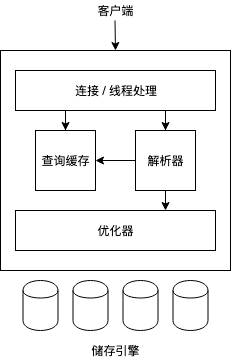
\includegraphics[width=0.4\textwidth]{db1.png}
    \caption{MySQL 架构分析图}
    \label{fig:db1}
\end{figure}


\subsection{数据库事务}

数据库事务是用户定义的一个数据库操作序列,是不可分割的工作单位。事务具有四个特征,分别是原子性:一个事务是不可分割的,事务内所有操作的状态必须一致;一致性:事务的作用必须使数据库从一个一致状态变为另一个一致状态;隔离性:多个事务的执行互不干扰;持续性:事务对数据库的修改是永久的。数据库事务是在并发条件下保证数据库数据正确的总要条件。

\subsection{MySQL 原理}
MySQL 是一个开源的关系型数据库管理系统。MySQL 非常的灵活,可以适应多种运行场景,例如:MySQL 既可以嵌入在程序中运行也可以支持数据仓库、在线处理系统等应用\cite{姜承尧2011mysql}。MySQL 主要由两部分组成:客户端与服务端。客户端的作用是向数据库系统发出命令并获取命令执行结果。服务端就是数据库系统本身,负责处理查询语句、执行查询并将查询结果返回客户端。

MySQL 是一个层次化系统,如图 \ref{fig:db1} 所示,主要包括 SQL 接口、查询 MySQL 解析器、MySQL 查询优化器以及查询执行引擎、缓冲/缓存机制和一个插件式的储存引擎。第二层服务是 MySQL 的核心,第三层则包括了储存引擎,它负责数据库中数据的储存与提取。我们可以根据需要选择不同功能的查询引擎\cite{schwartz2012high}。


MySQL 默认的库表结构与查询优化是不能有效地满足应用性能需求的,为此,我们需对 MySQL 的运行过程进行合理地优化。为了实现 MySQL 的高性能运行,我们需要对 MySQL 进行查询优化、索引优化以及库表结构优化。库表结构优化指为数据库选取合适的数据类型、合理使用 MySQL 特性、使用枚举类型以及使用缓存等操作。索引优化指在数据库表中的某些列上添加正确的索引翼加快查询速度。查询优化指合理设置查询方式,使得查询产生的中间结果最少、查询过程合理使用索引以及物理结构,使得查询速度加快。

\subsection{数据库设计原理}

本项目中采用基于 E-R (Entity - Relation, 实体 - 关系) 模型的设计方法进行设计。如图 \ref{fig:db2} 所示,数据库设计主要分为六个阶段:需求分析、概念设计、逻辑设计、物理设计、数据库实施以及数据库运行与维护\cite{王珊2006数据库系统概论}。

\begin{figure}[!ht]
    \centering
    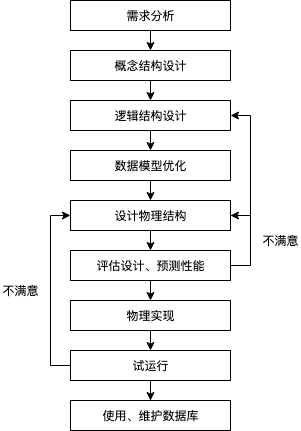
\includegraphics[width=0.4\textwidth]{db2.png}
    \caption{数据库设计流程图}
    \label{fig:db2}
\end{figure}

设计数据库时,首先必须分析设计需求,需求分析过程是整个设计的基础。随后,在需求分析的基础上开始概念结构设计,产出数据库概念结构。完成概念设计后,进行逻辑结构设计,将概念模型转换为数据库管理系统支持的逻辑模型,并进行优化。随后进行物理结构设计,即为设计好的逻辑结构选取最合适的物理结构。物理结构设计完成后,使用数据库语言建立相应的数据库、调试并进行数据入库。完成上述过程后,数据库即可开始运行,在运行时需根据实际情况作出调整与适当地维护\cite{wiederhold1983database}。


\section{视频编码}

在网络上进行传输的视频必须经过编码与压缩。网络传输的高清视频分辨率通常为 1920 $\times$ 1080,帧率为 30 帧,这样的视频如果不进行编码与压缩,一秒钟的视频产生文件大小为 177M 字节,移动网络大部分情况都不能以如此高的速率加载视频。因此要对视频进行编码与压缩,以某种方式压缩视频的算法称为视频编码。

目前主流的视频编码有 h.264\cite{richardson2004h} 和 h.265\cite{万帅2014新一代高效视频编码} 编码。h.264 编码比较成熟与稳定,目前所有的移动设备均能流畅解码播放,兼容性较好同时其编码器效率较高,编码速度较快,同时 h.264 编码的缺陷在于压缩率不如 h.265 编码。h.265 编码是最新的视频编码,h.265 编码的压缩率较高,h.265 编码视频只需使用 h.264 编码视频码率的一般即可达到同样的画质效果。h.265 编码的缺陷在于兼容性不如 h.264 编码,且编解码所需时间较长。

视频编码常用压缩算法主要有帧间压缩和帧内压缩。帧内压缩就是将视频的每一帧图像都进行有损压缩,如 Jpeg 压缩。其基本原理为应用人眼对亮度敏感同时对色彩不敏感的特性,尽可能保留图像的亮度信息,大幅压缩图像的色彩信息,以减小图像的大小。帧间压缩的原理是不保存视频所有的帧,只保留视频的关键帧以及两个关键帧之间像素的变化情况。帧间压缩通常采用帧间预测编码来实现\cite{richardson2004h}。

\begin{figure}[!ht]
    \centering
    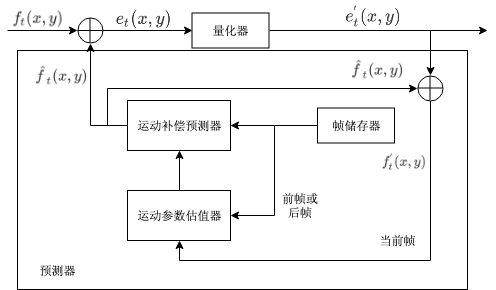
\includegraphics[width=0.6\textwidth]{video1.png}
    \caption{单向预测帧间编码}
    \label{fig:video1}
\end{figure}

帧间预测编码的基础是单向预测算法。单向预测算法通常将视频整个画面划分为若干块,以块为单位分配运动矢量\cite{毕厚杰2005新一代视频压缩编码标准}。具体预测过程如图 \ref{fig:video1} 所示,把当前帧 $f_{t}^{'})(x,y) $ 与前一帧 $f_{t-1}(x,y)$ 输入运动参数估计器中,运算后得到运动矢量,运动矢量输入补偿器得到预测图像 $\hat{f}_{t}(x,y)$。利用上一帧图像与运动矢量得到当前图像的算法称为单向预测算法:

\begin{equation}
\label{eq:forward_pre}
\hat{f}_{t}(x,y) = f_{t}(x+i, y+i)
\end{equation}

其中,$(i, j)$ 为运动矢量。目前通常采用基于单向预测算法的双向预测算法,即同时利用前一帧图像与后一帧图像进行预测:

\begin{equation}
\label{eq:forward_back_pre}
\hat{f}_{t}(x,y) = \alpha_{t-1}f_{t}(x+i, y+i) + \alpha_{t+1}f_{t}(x+i^{'}, y+i^{'})
\end{equation}

双向预测算法不可用于实时视频当中,只能用于实现录制好播放的视频中。

h.264 编码的视频中主要包含三种类型的帧:I 帧、P 帧以及 B 帧,表示运动补偿形式的不同。其中,I 帧为帧内编码帧也叫关键帧,保留完整的图像信息,对于视频进度条跳转有很大帮助。P 帧为帧间预测编码帧,且只能前向预测,它只参考前面最靠近它的I帧或者P帧。B 帧也是帧间预测编码帧, 它可以双向预测。每一个 I 帧以及它与下一个 I 帧之间所有的 P 帧与 B 帧称为一个 GOP 序列。B 帧的压缩率最大,解码的性能也最差,大量使用 B 帧可以节省空间放入更多的 I 帧,相同码率下画质会更好。因此在编码时要合理地设置 GOP 序列大小以及 B 帧的使用\cite{richardson2004h}。

\subsection{数据库与视频编码优化评价标准}
\subsubsection{数据库优化评价标准}
MySQL 主要测试指标有:吞吐量、响应时间、并发性以及可扩展性。吞吐量是指数据库每秒处理的事务的数量。数据吞吐量对于有大量用户同时访问的应用系统来说十分重要,直接决定系统的承载能力,常用测试单位为每秒事务数 (TPS)。响应时间指数据库系统完成一个任务所需要的平均时间,响应时间过长会造成数据库并发瓶颈,通常使用百分比响应时间 (percentile response time, PRT) 作为单位。并发性指数据库系统允许多少请求同时访问,通常测试并发数增加与吞吐量变化的关系。可扩展性指数据库系统在数据量增大时,能否增强其处理能力的特性\cite{schwartz2012high}。

\subsubsection{视频编码评价标准}

视频编码的评价标准主要有编码后视频的体积、编码时间、编码硬件占用以及某一码率下视频画质。编码后视频体积 ($V_{encoding}$) 表示了当前编码器设置的压缩率好坏。编码所用时间 ($T_{encoding}$) 表示编码一段短视频耗费时间,视频编码时间不能过长。编码硬件占用率 ($CPU_{encoding}$) 表示在编码时编码器对于 CPU 的占用情况,若过大,会造成服务器无力处理其他服务的情况。视频画质表示码率一定时不同编码方案的画质好坏,采用峰值信噪比 ($PSNR$) 作为单位\cite{毕厚杰2005新一代视频压缩编码标准},计算方法:

\begin{equation}
\label{eq:forward_back_pre}
PSNR_{dB} = \frac{10log_{10}(2^{n} - 1)^{2}}{MSE}
\end{equation}

其中 $MSE$ 为原始视频与编码后视频图像之间的均方误差,n 为每个像素的比特数。







